

\documentclass{article}
\usepackage[french]{babel}
\usepackage[letterpaper,top=2cm,bottom=2cm,left=3cm,right=3cm,marginparwidth=1.75cm]{geometry}
\usepackage{amsmath}
\usepackage{graphicx}
\usepackage{enumitem}
\usepackage[colorlinks=true, allcolors=blue]{hyperref}

\title{Projet 3 IA: Réseaux Bayésiens}
\author{Berthion Antoine - 566199}

\begin{document}


\maketitle

\section{Introduction}

\noindent Ce rapport a pour objectif d'explorer la stratégie d'implémentation d’un réseau bayésien pour la localisation de gemmes sur une carte à l’aide de données issues d’un sonar bruité. Nous y aborderons les défis liés à la complexité algorithmique de cette approche ainsi que les possibilités d’optimisation. En particulier, nous examinerons les axes d’amélioration en termes de réduction du temps d'exécution et d’augmentation de l'efficacité du modèle, afin d’obtenir des résultats précis tout en minimisant les ressources computationnelles nécessaires.

\begin{figure}[h]
    \centering
    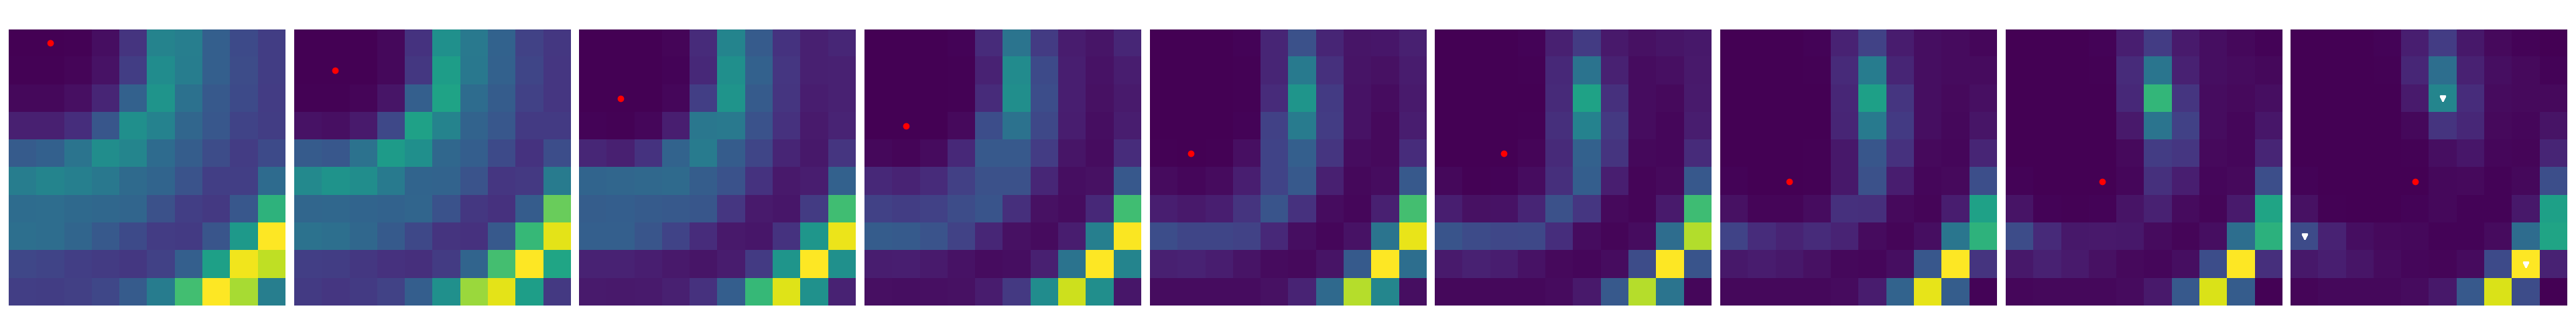
\includegraphics[width=1\textwidth]{src/intro.png}
    \caption{Résolution du problème exemple de l'énoncé}
    \label{fig:intro}
\end{figure}

\section{Implémentation}

\noindent Cette section se concentrera sur l’implémentation du projet, en détaillant les fonctions essentielles nécessaires à l’application de la technique d'inférence par énumération. Nous examinerons les composants clés de cette méthode, en expliquant leur rôle spécifique dans le processus d'inférence et leur contribution à l'atteinte des objectifs du projet.

\subsection{Fonction de vraisemblance} \label{sec:vraisemblance}

\noindent Après avoir obtenu les mesures de distances \( o_{i,j} \) à l'aide de notre sonar, l'objectif est de déterminer les positions \( P_{x,y} \) susceptibles d'avoir généré ces observations, et ainsi d'identifier les positions \( G_m \) correspondant aux gemmes. Pour ce faire, nous avons besoin d'une fonction permettant d'évaluer la vraisemblance entre une observation \( o_{i,j} \) et l'observation théorique associée à une position potentielle \( P_{x,y} \), notée \( o_{x,y} \). 

\vspace{1em}

\noindent Nous définissons la distance \( d \) entre \( o_{i,j} \) et \( o_{x,y} \) comme suit :

\[
d = \left| o_{i,j} - o_{x,y} \right|
\]

\noindent Il convient désormais de noter que plus \( d \) est proche de zéro, plus la position \( P_{x,y} \) est vraisemblablement celle d'une gemme. Inversement, à mesure que \( d \) augmente, la probabilité que \( P_{x,y} \) soit une gemme diminue. Afin de quantifier cette vraisemblance, nous souhaitons utiliser une fonction qui renvoie une valeur tendant vers 1 lorsque la vraisemblance est maximale et tendant vers 0 lorsqu'elle est minimale. Nous posons donc l'équation suivante pour la vraisemblance :

\[
likelihood = 2^{-d}
\]

\vspace{1em}

\noindent Ainsi, lorsque \( d \) tend vers 0, la vraisemblance tend vers 1, indiquant que la position est très probablement une gemme. Le choix de la base 2 dans cette fonction est arbitraire ; toutefois, plus la base est grande, plus l'impact de la distance \( d \) sera significatif, rendant la vraisemblance plus sensible aux écarts de distance.

\subsection{Fonction d'inférence énumérative}

\noindent Étant désormais muni de la fonction de vraisemblance discutée dans la section \ref{sec:vraisemblance}, nous allons discuter de la stratégie d'inférence par énumération que nous allons mettre en place. 

\vspace{1em}

\noindent Nous allons itérer à travers l'ensemble des permutations possibles de \( m \) gemmes, pour notre grille \( n \times n \) (\( n^2 \) positions disponibles). Notons que ce nombre de permutations est dénombrable, et se calcule :

\[
P(n^2, m) = \frac{(n^2)!}{(n^2 - m)!}
\]

\vspace{1em}

\noindent Pour chacune de ces permutations, nous souhaitons évaluer à quel point il est vraisemblable que ces \( m \) positions soient les positions de nos gemmes. Nous faisons alors appel à la fonction de vraisemblance énoncée plus tôt. Nous allons dès lors ajouter cette vraisemblance aux \( m \) positions \( x, y \) dans une matrice \textit{posterior}. De ce fait, les permutations vraisemblables feront augmenter les cases probables, et les cases peu probables resteront proches de 0.

\noindent Nous combinerons finalement cette matrice \textit{posterior} avec notre matrice de croyances. Ainsi, au fur et à mesure des itérations, notre réseau de Bayes deviendra de plus en plus certain des positions des gemmes. En effet, chaque changement de positions générera de nouveaux vecteurs d'observations, qui viendront renforcer et corroborer les croyances préexistantes.

\subsubsection{Complexité}\label{subsec:complex}

\noindent Nous allons désormais montrer que la complexité de l'algorithme d'énumération présenté est de l'ordre de \( \mathcal{O}(n^{2m}) \). Examinons le nombre de permutations \( P(n^2, m) \) de \( m \) éléments parmi \( n^2 \) positions.

\vspace{1em}

\begin{enumerate}[left=0pt]

\item \textbf{Expression exacte du nombre de permutations} \\
Comme discuté précédement, le nombre total de permutations \( P(n^2, m) \) de \( m \) éléments parmi \( n^2 \) positions est donné par :
\[
P(n^2, m) = \frac{(n^2)!}{(n^2 - m)!}
\]

\item \textbf{Développement en produit de termes} \\
Ce nombre peut être réécrit comme le produit des \( m \) premiers termes de \( (n^2)! \), puisque nous ne prenons que \( m \) éléments parmi \( n^2 \). Donc :
\[
P(n^2, m) = (n^2) \times (n^2 - 1) \times (n^2 - 2) \cdot \dots \times (n^2 - m + 1) = \prod_{k=0}^{m-1} (n^2 - k)
\]

\item \textbf{Majoration de chaque terme} \\
Puisque chaque facteur du produit \( (n^2 - k) \) pour \( k = 0, 1, \dots, m-1 \) est au maximum \( n^2 \), nous avons :
\[
\prod_{k=0}^{m-1} (n^2 - k) \leq \underset{\text{m termes}}{\underbrace{(n^2) \times (n^2) \times \dots \times (n^2)}}
= (n^2)^m = n^{2m}
\]

\item \textbf{Conclusion} \\
Il en ressort que le nombre de permutations \( P(n^2, m) \) est borné par \( n^{2m} \). Étant donné que l'algorithme ne réalise que des opérations de coût constant pour chaque permutation (calcul de la distance euclidienne et évaluation de la vraisemblance), la complexité asymptotique dépend uniquement de cette borne supérieure des permutations \( P(n^2, m) \), ce qui conduit à la complexité asymptotique suivante :
\[
\mathcal{O}(n^{2m})
\]

\end{enumerate}

\noindent Il convient de souligner que cette complexité est de nature exponentielle, ce qui est attendu, étant donné que l'algorithme appartient à la classe des algorithmes naïfs.



\section{Expérimentations}

\noindent Dans cette section du rapport, nous analyserons les défis computationnels associés à la nature exponentielle de notre algorithme (\ref{subsec:complex}), en fonction du nombre \( m \) de gemmes et de la taille \( n^2 \) de la grille.

\vspace{1em}

\noindent Nous allons évaluer la performance computationnelle en mesurant le temps nécessaire pour effectuer une unique inférence dans une grille de dimensions \( n \times n \) contenant \( m \) gemmes. Les résultats de cette analyse sont présentés ci-dessous dans la figure \ref{fig:exp_inf}.

\begin{figure}[h]
    \centering
    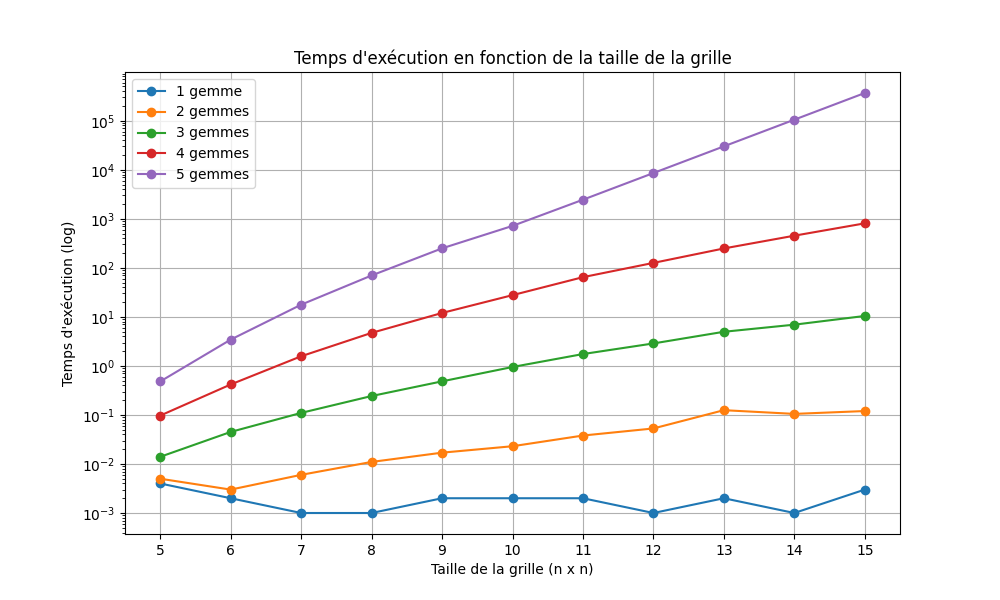
\includegraphics[width=0.9\textwidth]{src/exp.png}
    \caption{Temps d'exécution d'une inférence unique}
    \label{fig:exp_inf}
\end{figure}

\noindent Nous observons que les comportements suivent effectivement une tendance exponentielle, comme en témoigne la linéarité des courbes sur un graphique à échelle logarithmique. Les temps d'exécution deviennent suffisamment élevés pour qu'au-delà d'une grille de dimensions \( 12 \times 12 \) avec 5 gemmes, il ait été nécessaire d'interpoler les résultats.

\section{Optimisations}

\noindent Dans cette section, nous discuterons des améliorations potentielles de notre algorithme d'inférence par énumération. Nous allons aborder des techniques permettant de diminuer la complexité de l'algorithme. Nous ne pourrons néanmoins pas rendre l'inférence par énumération polynomiale.

\subsection{Utilisation des combinaisons}

\noindent Il est en réalité inutile d'employer les permutations dans notre approche. En effet, il est possible de trier d'abord le vecteur des observations \( o_{i,j} \), puis de trier le vecteur des observations \( o_{x,y} \), afin d'assurer une comparaison correcte des vraisemblances des gemmes correspondantes.

\vspace{1em}

\noindent En recourant aux combinaisons, nous réduisons efficacement le nombre d'ensembles de gemmes à vérifier à l'aide de la fonction de vraisemblance. Ce nombre peut être dénombré comme suit :
\[
\binom{n^2}{m} = \frac{(n^2)!}{(n^2 - m)! \cdot m!}
\]
Ainsi, cette approche permet de réduire le nombre total de comparaisons à effectuer.

\subsection{Élimination des zones invraisemblables}

\noindent Afin d'éviter de générer des permutations dont l'invraisemblance est déjà établie, nous pouvons éliminer ces positions avant de procéder au calcul des permutations.

\vspace{1em}

\noindent Nous introduisons ainsi \( \varepsilon \), le seuil en dessous duquel les cases seront rejetées. En supposant que \( k \) cases soient invraisemblables, c'est-à-dire que \( \textbf{likelyhood}(k) \leq \varepsilon \), nous obtenons alors \( n^2 - k \) positions possibles. En termes de combinaisons, cela se traduit par :
\[
\binom{n^2 - k}{m} = \frac{(n^2 - k)!}{(n^2 - k - m)! \cdot m!}
\]

\noindent De cette manière, nous éviterons de recalculer des vraisemblances faibles à plusieurs reprises. Il convient de souligner que \( \varepsilon \) doit être judicieusement choisi afin de ne pas négliger des cases qui, bien que présentant un score de vraisemblance faible, pourraient être affectées par le bruit du sonar. 

\section{Utilisation des LLM}

\noindent Dans cette courte partie, nous discuterons de l'utilisation des LLM dans le cadre du projet. Aucun LLM n'a été utilisé pour l'aspect implémentation ainsi que la compréhension du projet. Cependant, ce rapport à été corrigé du point de vue de la syntaxe et de la grammaire par DeepL ainsi qu'un modèle GPT. Notons tout de même qu'aucune des informations du rapport n'a été produite par une autre personne que l'auteur.

\section{Conclusions}

\noindent En conclusion, ce projet a permis de mettre en œuvre et d’analyser un réseau bayésien pour la localisation de gemmes sur une grille à partir de données de sonar bruitées. Nous avons détaillé les étapes clés de l’implémentation, y compris la définition de la fonction de vraisemblance et la mise en place de l’inférence par énumération. À travers cette approche, nous avons démontré que la complexité de l’algorithme suit une croissance exponentielle, ce qui limite sa scalabilité, notamment pour des grilles de grandes tailles ou un grand nombre de gemmes.

\vspace{1em}

\noindent Les expérimentations ont révélé un comportement exponentiel des temps d’exécution, confirmant l'impact de la croissance combinatoire du nombre de permutations à traiter. Cela nous a amenés à envisager des optimisations, telles que l’utilisation des combinaisons et l’élimination des zones invraisemblables, pour réduire la complexité et améliorer l’efficacité de l’algorithme. Malgré ces améliorations, la nature exponentielle de l’algorithme reste inchangeable et représente une limite majeure de l'inférence par énumération.

\end{document}